\documentclass[12pt,a4paper]{article}
\usepackage[latin1]{inputenc}
\usepackage{graphicx}
\usepackage[margin=1in]{geometry}
\DeclareGraphicsExtensions{.png,.eps,.jpg}

\author{Navy Team}

\title{\LARGE NavUP : Software Requirements Specification}

\begin{document}

	\maketitle

	\begin{flushright}
	 \textbf{Team Members: }\newline
	 Claudio Da Silva 14205892\newline
	 Ruan Klinkert \newline
	 Regan Koopmans 15043143\newline
	 Tlou Lebelo 15209190\newline
	 Lindelo Mapumulo 12002862\newline
	 Nkosinathi Mothoa 12077420\newline
    \end{flushright}

	\pagebreak
	\tableofcontents
	\pagebreak


	\section{Introduction}

		\subsection{Purpose}

		The goal of this Software Requirements Specification is to ascertain the
		concrete necessities that the proposed software, NavUP, should fulfil. This
		software, amongst other tasks, will act primarily as a navigation tool. For
		this reason we believe the two main interest groups are:

		\begin{itemize}
			\item Students who are search for a particular building on campus, or are
						investigating the many historically relevant buildings on campus.

			\item Guests to the university that require assistance finding locations.
		\end{itemize}


		\subsection{Scope}

			The system proposed will be called NavUP. Put briefly, the product will
			on-campus navigation support to students, lecturers, and visitors to
			the university. This software will create value for the end user, in that
			it solves the problem of finding specific locations on campus better than
			the current solution of static maps and written descriptions. This
			necessity is particularly accute in first-year students and guests to the
			university, where the lack of such knowledge creates anxiety, stress and
			occupies time and mental energy that might be better spent otherwise.

		\subsection{Definitions, Acronyms and Abbreviations}

		\subsection{References}

		\subsection{Overview}

			This SRS document is structured...

	\section{Overall Description}

		The NavUP Navigation system

		\subsection{Product Perspective}

			\subsubsection{System Interfaces}

			\subsubsection{User Interfaces}

				There will be three main mediums through which prospective users can
				interact with the proposed system. These are:

				\paragraph{Web Interface}

					Users will be able to access the software through an intuitive Web
					Interface, and hence through any device that has an up-to-date browser.

				\paragraph{Android Application}

					An Android application will allow the users of Android smartphones
					and tablets to interact with the system with a native application on
					their device.

				\paragraph{iOS Application}

					An iOS application, similarly to the Android app, will enable mobile
					Apple devices, such as iPhones or iPads, to connect to the software
					service.

			\subsubsection{Hardware Interfaces}

				As described above, we intend to publish to three platforms.

			\subsubsection{Software Interfaces}



			\subsubsection{Communication Interfaces}

			\subsubsection{Memory}

				Most information regarding the system will reside in a central
				database. This database will contain, amongst other things:

				\begin{itemize}
					\item User information
					\item Locations
					\item Events
					\item Route caching
				\end{itemize}

				For network efficiency, it will make sense to keep a portion of this
				data locally on the device in question. Similarly the browser may store
				a small fraction of this data (most likely user data) to reduce data
				usage, server strain and lookup time.

			\subsubsection{Operations}



			\subsubsection{Site Adaptation Requirements}

				The system will need to be able to adapt to the changing environment of
				the university. The system should be able to acknowledge a change in the
				WiFi-topology, and changes in the physical layout of the university, and
				use this new information to in the paths that it is generating for the
				users.


				The product should idealy be as decoupled from UP as possible. In doing
				this, the product might be deployed elsewhere with minimal modification,
				and therefore make the system more beneficial than simply it usage in
				the university.


		\subsection{Product Functions}

			\begin{itemize}
				\item Successfully identify a user's current location, and plan an
							accurate route to another location on campus.
			\end{itemize}

		\subsection{User Characteristics}

			For the average user of the system we should not assume any more technical
			skills than that required to operate simple smartphone apps. The proposed
			software should imitate, as far as possible, the paradigms and ideologies
			that previous mobile and browser applications have established. We can
			expect that students will have encountered navigational systems such as
			Google Maps, and should thus try to meet the expectations that users have
			developed in using these application.

		\subsection{Constraints}

			\begin{itemize}

				\item We do not need to account for navigation off-campus
				\item We can only accurately navigate within sufficient WiFi coverage.

			\end{itemize}

		\subsection{Assumptions and Dependencies}



	\section{Specific Requirements}

		\subsection{External Interface Requirements}

			\paragraph{The system will interface with WiFi Hardware}

				The system will poll a request to the hardware by giving a access point
				address, and will hopefully return a floating point number between 0 and
				 1 describing how strong the signal the this access point is. It may be
				 possible that the Android and iOS APIs provide enough expressiveness
				 that we do not actually need to concern ourselves with hardware
				 details, but purely network primitives. This will have to be a fast
				operation, as we anticipate this will occur for every access point in
				the vacinity at least once a second, preferably more.


		\subsection{Functional Requirements}


			\textbf{The NavUPlocation Module} \newline \newline
			The NavUPlocation module provides all the functionality directly related to the navigation aspect of NavUP. 					Services in this module may be used in other modules to further improve the user's general experience.

			\medskip

			\begin{figure}[h!]
				\centering{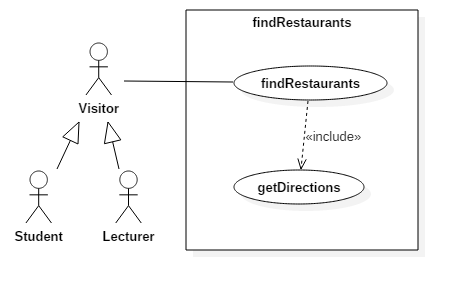
\includegraphics[width=0.7\linewidth]{images/findRestaurants.png}}
				\caption findRestaurants use case diagram.
			\end{figure}

			\textbf{findRestaurants}
			The following use case locates all the restaurants in the university's campus, and then provides a detailed list 				view for the user. The details include the name, dietary requirements served and a link to navigate to the 						restaurant from current location.

			\begin{itemize}
			\item Pre-condition: The user must have a phone with location services, and must have location functionality        				  enabled for the mobile application.
			\item Post-condition: The user is presented with a detailed list of all restaurants on campus. From here, they can 				  choose to navigate to the selected restaurant.
			\end{itemize}

			\textbf{findRestrooms}
			The following use case locates all the restrooms on campus, and then lists them to the user. The list provides     			options to navigate to the nearest restrooms (relative to the user's current location).

			\begin{itemize}
			\item Pre-condition: The user must have a phone with location services, and must have location functionality  						  enabled for the mobile application.
			\item Post-condition: List of restrooms is presented to the user. This list also includes an option that will 						  allow the user to navigate to the nearest restroom.
			\end{itemize}

			\begin{figure}[h!]
				\centering{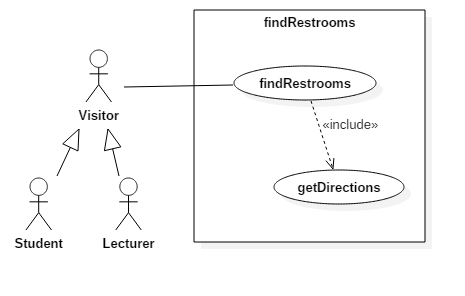
\includegraphics[width=0.7\linewidth]{images/findRestrooms.png}}
				\caption findRestrooms use case diagram.
			\end{figure}

			\textbf{findExitsAndEntrances}
			The following use case locates all the entrances and exits on campus. A detailed list (which includes the type of 				exit or entrance - pedestrian or vehicle - is provided to the user). The list also provides an option for the user 			to navigate to the exit or entrance, from their current location.

			\begin{itemize}
			\item Pre-condition: The user must have a phone with location services, and must have location functionality 						  enabled for the mobile application.
			\item Post-condition: A list of all the entrances and exits is provided to the user. From this list, a user can 					  also choose to navigate to the exit or entrance, from their current location.
			\end{itemize}

			\begin{figure}[h!]
				\centering{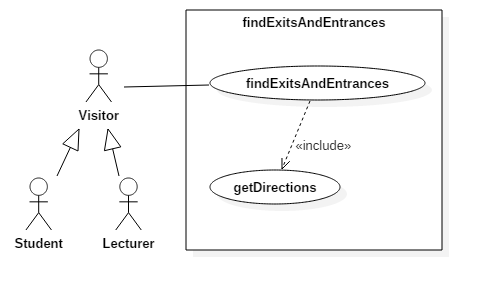
\includegraphics[width=0.7\linewidth]{images/findExitsAndEntrances.png}}
				\caption findExitsAndEntrances use case diagram.
			\end{figure}

			\textbf{findBuilding}
			The following use case finds a building for the user. The user is provided with the building location and an 					option to navigate to the building.

			\begin{itemize}
			\item Pre-condition: The user must have a phone with location services, and must have location functionality 						  enabled for the mobile application. The user also needs to provide the name for the building in order for 					  the building to be located.
			\item Post-condition: A list of buildings that match the user's text search are returned. The list also provides   				  the user with an option to navigate to the building, from their current location.
			\end{itemize}

			\begin{figure}[h!]
				\centering{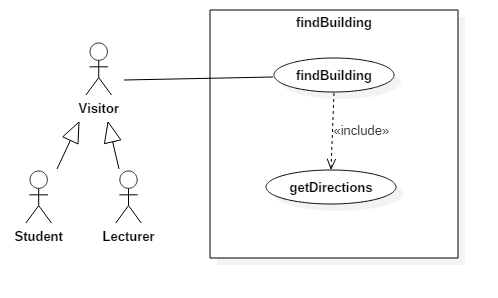
\includegraphics[width=0.7\linewidth]{images/findBuilding.png}}
				\caption findBuilding use case diagram.
			\end{figure}

			\textbf{listBuildings}
			The following use case lists all the buildings on campus. From there a user has the option to navigate to the 					selected building, from their current location.

			\begin{itemize}
			\item Pre-condition: The user must have a phone with location services, and must have location functionality 						  enabled for the mobile application.
			\item Post-condition: List of buildings on campus is provided to the user. User can also navigate to selected   					  building.
			\end{itemize}

			\begin{figure}[h!]
				\centering{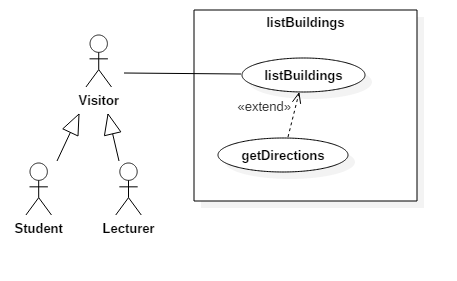
\includegraphics[width=0.7\linewidth]{images/listBuildings.png}}
				\caption listBuildings use case diagram.
			\end{figure}

			\textbf{findLectureRoom}
			The following use case finds a lecture room in the building the user is currently located. User can navigate to 				that lecture room, given their current location in the same building.

			\begin{itemize}
			\item Pre-condition: The user must have a phone with location services, and must have location functionality 						  enabled for the mobile application. The user must be in the building of the lecture room they are trying 						  to find.
			\item Post-condition: A detailed list of lecture room results is presented to the user. This list also makes it 					  possible for the user to navigate to the lecture room.
			\end{itemize}

			\begin{figure}[h!]
				\centering{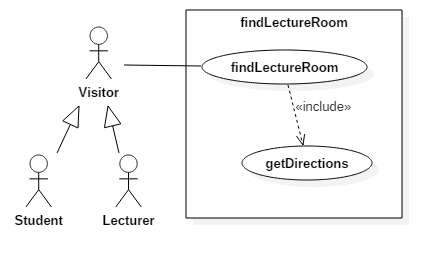
\includegraphics[width=0.7\linewidth]{images/findLectureRoom.png}}
				\caption findLectureRoom use case diagram.
			\end{figure}

		    \textbf{listBuildingsLectureRooms}
            The following use case lists all the lecture rooms in the building the user is currently located. User can              	        navigate to any selected lecture room, given their current location in the same building.

			\begin{itemize}
			\item Pre-condition: The user must have a phone with location services, and must have location functionality 			              enabled for the mobile application. User must be in a building to list lecture rooms for that building.
			\item Post-condition: A detailed list of all the lecture rooms in the current building is presented to the user. 					  This list also makes it possible for the user to navigate to the lecture room.
			\end{itemize}

		    \textbf{getCurrentLocation}
			The following use case gets the current location of the user and views the details (if available) about the 		            current location.

			\begin{itemize}
			\item Pre-condition: The user must have a phone with location services, and must have location functionality 			              enabled for the mobile application.
			\item Post-condition: The current location and its details are displayed to the user.
			\end{itemize}

	        \textbf{getDirections}
			The following use case gets directions from one location on campus to another within the university campus.

			\begin{itemize}
			\item Pre-condition: The user must have a phone with location services, and must have location functionality 						  enabled for the mobile application. Two distinct locations (to and from) within the campus premises need to        			      be selected.
			\item Post-condition: Directions between two locations are presented to the user.
			\end{itemize}

			\begin{figure}[h!]
				\centering{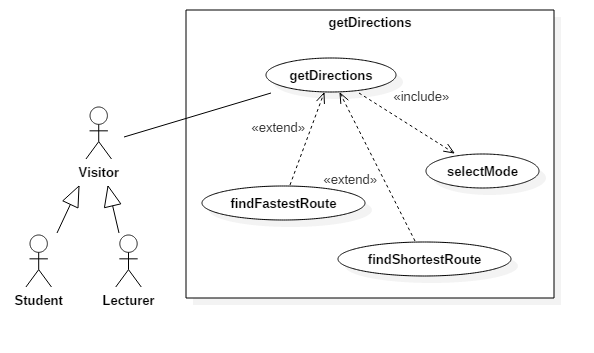
\includegraphics[width=0.7\linewidth]{images/getDirections.png}}
				\caption getDirections use case diagram.
			\end{figure}

		    \textbf{findFastestRoute}
			The following use case finds the fastest route between two campus locations. Time is affected by congestion on 				    walkways and/or campus roads.

			\begin{itemize}
			\item Pre-condition: The user must have already selected two distinct locations on campus (to and from), and have 					  already requested directions using \textit{getDirections}.
			\item Post-condition: The directions for the fastest route between two locations are presented to the user.
			\end{itemize}

			\textbf{findShortestRoute}
			The following use case finds the shortest route between two campus locations. Distance is only limited to the 				    horizontal distance a user has to travel (i.e. floor elevation is not considered).

			\begin{itemize}
			\item Pre-condition: The user must have already selected two distinct locations on campus (to and from), and have 					  already requested directions using \textit{getDirections}.
			\item Post-condition: The directions for the shortest route between two locations are presented to the user.
			\end{itemize}

			\textbf{selectMode}
			The following use case allows a user to select a mode of transport in order to find best routes for the mode of 		        transportation.

			\begin{itemize}
			\item Pre-condition: The user must have already selected two distinct locations on campus (to and from), and have 					  already requested directions using \textit{getDirections}.
			\item Post-condition: The directions for selected mode of transportation between two locations are presented to     				  the user.
			\end{itemize}

	    \textbf{The NavUPacademic Module} \newline

	    The \textit{NavUPacademic} module provides students and lecturers with enhanced \textit{NavUPlocation} services to 				improve their general navigation throughout the university's campus. Visitors do not have access to any of the 				    services found in this module.

	    \medskip

	    \textbf{uploadStudentTimetable}
		The following use case enables a user to upload or update their student timetables (lectures, practical sessions, 			    tutorial sessions, examinations and semesters tests).

		\begin{itemize}
		  \item Pre-condition: User must have selected the student option under the usage modes (\textit{selectUsageMode}). 					User must also be logged in.
		   \item Post-condition: Uploads or updates the user's student timetable.
		\end{itemize}

	    \textbf{viewStudentTimetable}
		The following use case enables a user to view their student timetables (lectures, practical sessions, tutorial        			sessions, examinations and semesters tests).

		\begin{itemize}
		  \item Pre-condition: User must have selected the student option under the usage modes (\textit{selectUsageMode}). 					User must have already uploaded their student timetables, and logged in.
		   \item Post-condition: Views the user's student timetable.
		\end{itemize}

	    \textbf{getNextStudentTimetableEvent}
		The following use case gets and then views the details of next event on the student's timetable. From there, a student 		has options to get directions to that event.

		\begin{itemize}
		  \item Pre-condition: User must have selected the student option under the usage modes (\textit{selectUsageMode}). 					Student must be logged in, and have already uploaded a timetable.
		   \item Post-condition: Details about the next event on the student's timetable are displayed. Student is also 						 provided with an option to get directions to the next event.
		\end{itemize}

		\begin{figure}[h!]
				\centering{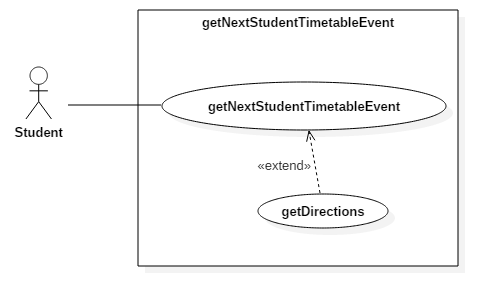
\includegraphics[width=0.7\linewidth]{images/getNextStudentTimetableEvent.png}}
				\caption getNextStudentTimetableEvent use case diagram.
		\end{figure}

		\textbf{uploadLecturerTimetable}
		The following use case enables a user to upload or update their lecturer timetables (lectures, consultations times and 		invigilation times).

		\begin{itemize}
		  \item Pre-condition: User must have selected the lecturer option under the usage modes (\textit{selectUsageMode}). 					User must also be logged in.
		   \item Post-condition: Uploads or updates the user's lecturer timetable.
		\end{itemize}

	    \textbf{viewLecturerTimetable}
		The following use case enables a user to view their lecturer timetables (lectures, consultations times and 		     		    invigilation times).

		\begin{itemize}
		  \item Pre-condition: User must have selected the lecturer option under the usage modes (\textit{selectUsageMode}). 			        User must have already uploaded their lecturer timetables, and logged in.
		   \item Post-condition: Views the user's lecturer timetable.
		\end{itemize}

	    \textbf{getNextLecturerTimetableEvent}
		The following use case gets and then views the details of next event on the lecturer's timetable. From there, a 			    lecturer has options to get directions to that event.

		\begin{itemize}
		  \item Pre-condition: User must have selected the lecturer option under the usage modes (\textit{selectUsageMode}). 		            Lecturer must be logged in, and have already uploaded a timetable.
		   \item Post-condition: Details about the next event on the lecturer's timetable are displayed. Lecturer is also 						 provided with an option to get directions to the next event.
		\end{itemize}

		\textbf{The NavUPadministration Module} \newline

		The \textit{NavUPadministration} module contains all the services that are related to the general administration of 			NavUP. These are accessible by users of any mode.

	    \medskip

	    \textbf{getHelp}
		The following use case provides a user with assistance on how the mobile application works, and where on the 				    university campus they can get assistance that is not related to the mobile application.

		\begin{itemize}
		  \item Pre-condition: None.
		   \item Post-condition: Provides users with locations where they can get assistance. Also provides users with 		  		             assistance on how to use the mobile application (in the form of FAQs).
		\end{itemize}

		\textbf{registerNewUser}
		The following use case allows a user to register to use the NavUP mobile application. Registration is only mandatory 			for students and lecturers who wish to make use of additional functionality. Visitors are not required to register.

		\begin{itemize}
		  \item Pre-condition: None.
		   \item Post-condition: A new NavUP account is created for the user.
		\end{itemize}

		\textbf{userLogin}
			The following use case allows a user to login to use the NavUP mobile application. Visitors are not required to 				login.

		\begin{itemize}
		  \item Pre-condition: User must be already registered to use NavUP.
		   \item Post-condition: User is logged in to NavUP if they provide correct login details.
		\end{itemize}

	    \textbf{selectUsageMode}
	    The following use case allows a user to select the mode(s) they would like to use the mobile application. Visitor mode    		may not be used in conjunction with other modes. Student and Lecturer modes can be used in conjunction (e.g. user is 			both a Master's Degree student and a lecturer).

		\begin{itemize}
		  \item Pre-condition: User must be logged in if using NavUP as a lecturer or student.
		   \item Post-condition: The usage mode is changed to the user's selection.
		\end{itemize}


		\subsection{Performance Requirements}

			The system will need to operate within reasonable levels of speed and
			responsiveness to be useful to the end-user. For this reason we will need
			to consider a path finding algorithm that is suited to both the need for
			accuracy and the time needed to calculate such a path.

			\medskip

			One strategy that we might use is to \textit{precompute portions of the
			path-finding}. We may already know the best route between two shorter
			paths, and hence the search space of the path finding algorithm can be
			greatly reduced when composed of only two or three path ``legs'' to choose
			from.

			\medskip

			Further, since the largest number of users is expected to be mobile users,
			criteria such as battery usage and processing power will be of
			great concern. To this end, we can think about caching the data that is
			most important and most frequently used for the user on their devices.
			This will make the system feel more responsive, and will reduce overall
			strain on the system.

			\medskip

			We can also think about caching on the system itself. If two students
			request a path to the same location, and are within 20 meters of one
			another, we can consider that as two equal requests and compute this once.
			The system can keep a log of requests within storage, for a limited period
			of time. This will save massive amounts of recomputation.

			\medskip

			In terms of accuracy, the software will need provide navigation between
			individual lecture halls. This means that an accuracy with less than a 5
			meter error is essential for insuring that lecture-hall resolution can
			still work reliably.

		\subsection{Design Constraints}

			The success and performance of the proposed system is contingent on the
			following citeria which cannot be altered:

			\paragraph{Accuracy Is Limited By Device}

				Due to the fact that navigation is dependent entirely on WiFi signal
				strength, the accuracy of the navigation can only ever be as proficient
				as the sensitivity of the WiFi hardware. This is a fundamental constraint,
				and cannot be worked around in the current vision of the proposed
				software.

			\paragraph{Processing Capability}

				Mobile devices vary significantly in terms of processing capability,
				particularly so in Android devices. In order to make the system
				available to the largest possible audience, we must build to the lowest
				common denominator. With this in mind, we must be confident that the
				application will run smoothly on a device that may only have a single
				500 Mhz processor. The only way to achieve this is to make the client
				application as light as possible, and only do essential processing on
				device itself.

				\paragraph{Navigation is Limited By Source Maps}

				The system's ability to navigate is directly proportional to the accuracy
				of the maps which we use. If the university has been poorly mapped in
				certain areas, navigation may be inaccurate or impossible altogether.

		\subsection{Software System Attributes}

			Another concern is the security of users' data. To prevent a compromise of
			private data we must follow the best practises as established by industry
			leaders, such as:

			\begin{itemize}
				\item Not storing plain text passwords
				\item Not storing identifying data points
				\item Encrypting critical data communication
				\item Maintaining anonymity as far as possible
			\end{itemize}

			This system will be available at all times, and a maintainer or
			administrator will only have to interact with the system when
			\textit{CRUD}-ing locations and events, or to observe usage statistics
			through the analytics dashboard.

			\medskip

			Value may also be extended by integrating third-party services. One such
			addition would be integration with \textit{Google Calendar}. From Google
			Calendar we would be able to get timed appointments at specific locations,
			and would therefore be able to find paths to these appointments before
			they were even requested by the user. Interoperability with the UP network
			services would equally be automatically load lecture times for both
			lecturers and students.

		\subsection{Other Requirements}

	\section{Traceability Matrix}

	The table below uses requirements (R) and uses cases (UC) as enumerated in
	\textit{3.2 Functional Requirements}.

	\begin{table}[!h]
		\centering
		\caption{Tracibility Matrix for Proposed Software}
		\label{my-label}
		\begin{tabular}{|ll|l|l|l|}
			\hline
			\multicolumn{1}{|l|}{Requirement} & Priority & UC1 & UC2 & UC3 \\ \hline
			\multicolumn{1}{|l|}{R01}            &          &     &     &     \\ \hline
			\multicolumn{1}{|l|}{R02}            &          &     &     &     \\ \hline
														&    UCPriority   &     &     &     \\ \hline
		\end{tabular}
	\end{table}

	\section{Appendix}

		\subsection{Abbreviated list of Use Cases}

			\begin{itemize}
				\item [\textbf{UC1}] Use case
			\end{itemize}

		\subsection{Abbreviated list of Requirements}

			\begin{itemize}
				\item [\textbf{R01}] Requirement
			\end{itemize}

\end{document}
